% ------------------------------------------
%  MASTER THESIS DISSERTATION
% ------------------------------------------
% Author:
%
% Advisors:
%
% ------------------------------------------
\documentclass[10pt,twoside,openright,a4paper]{report}
\usepackage[utf8]{inputenc}

% Set document margins to 1in in all sides
\usepackage[margin=2.5cm]{geometry}
% Line spacing package
\usepackage{graphicx, helvet, hyperref, setspace}
\usepackage[portuguese,english]{babel}
\usepackage[nomain, acronym, toc]{glossaries}
% Extra stuff file
% This file is included before begin{document} environment
% Use this to include extra packages and define your own commands
% This way, you can easily grab a most recent version
% of dissertation.tex file from the original repo


% Built the glossary when the main file is built.
\makeglossaries
% Set main font to Arial
\renewcommand{\familydefault}{\sfdefault}
% Define keywords macro
\providecommand{\keywords}[1]{\textbf{Keywords:} #1}
% Define "palavras-chave" macro
\providecommand{\palavrasChave}[1]{\textbf{Palavras-Chave:} #1}
% Define the NewPage macro
\newcommand*\NewPage{\newpage\null\thispagestyle{empty}\cleardoublepage}
% Abstract-en page numbering
\newcommand {\abstractEnglishPageNumber} {\thispagestyle{plain}\setcounter{page}{\abstractEnglishPage}}
% Abstract-pt page numbering
\newcommand {\abstractPortuguesePageNumber} {\thispagestyle{plain}\setcounter{page}{\abstractPortuguesePage}}
% Section numbering depth
\setcounter{secnumdepth}{3}
% Table of contents depth
\setcounter{tocdepth}{3}
% Set line spacing to 1.5cm
\onehalfspacing
% Page numbering
\pagestyle{plain}

% Glossary-File
% Glossary Definition

\newglossaryentry{MSc}{name={MSc}, description={Masters degree in the area of Science.}}

% Acronym-File
% Acronym Definition

\newacronym{IST}{IST}{Instituto Superior T\'ecnico}


% ------------------------------------------
% MASTER THESIS DISSERTATION
% ------------------------------------------

\begin{document}
\pagenumbering{gobble}% Remove page numbers (and reset to 1)
\clearpage
\thispagestyle{empty}
%!TEX root = ./dissertation.tex

% Dissertation basic information
\newcommand {\Title} {MIMBCD-UI}
\newcommand {\Subtitle} {Medical Imaging Multimodality Breast Cancer Diagnosis User Interface}
\newcommand {\StudentName} {Francisco Maria Calisto}
\newcommand {\DegreeName} {Computer Science and Engineering}
\newcommand {\Supervisors} {{\large Prof./Dr. Lorem Ipsum}}

% Include or not include acknowledgments
\def \includeAcknowledgments{1}

% Include or not include glossary
\def \includeGlossary{0}

% Examination Committee
\newcommand {\Advisor} {{\large Prof. Dr. Jacinto Nascimento}}
\newcommand {\CoAdvisor} {{\large Prof. Dr. Daniel Gon\c{c}alves}}

% After the thesis defense
\newcommand {\CommitteeMembers} {
{\large Prof./Dr. Lorem Ipsum}\\
{\large Prof./Dr. Lorem Ipsum}
}
\newcommand {\Chairperson} {{\large Prof./Dr. Lorem Ipsum}}

% Is final version (will include Committee Members information)
\def \IsFinalVersion{1}

% Date
\newcommand {\Month} {October}
\newcommand {\Year} {2017}

% Acknowledgments page number
\def \acknowledgmentsPage{1}

% Abstract-en page numbering
\def \abstractEnglishPage{3}

% Abstract-pt page number
\def \abstractPortuguesePage{5}

% You had a co-advisor:
\def \HasCoAdvisor{0}

% Logo Spacing Variables
\def \finalLogoSpacing{2.0cm}
\def \draftLogoSpacing{2.0cm}

% Advisors Spacing Variables
\def \finalAdvisorsSpacing{1.0cm}
\def \draftAdvisorsSpacing{10.0cm}

% Date Spacing Variable
\def \dateSpacing{5.0cm}

% You can define your own variables here


%!TEX root = ./dissertation.tex

% ---------------------------------------------------------
%   MASTER THESIS DISSERTATION COVER
% ---------------------------------------------------------
\begin{titlepage}
% ---------------------------------------------------------
%  INSTITUTION LOGO
% ---------------------------------------------------------

\includegraphics[width=5cm]{images/ist_logo}~\\
%
\if\IsFinalVersion 1
  \vspace*{\finalLogoSpacing}
\else
  \vspace*{\draftLogoSpacing}
\fi

\begin{center}
% ---------------------------------------------------------
%  MASTER THESIS DISSERTATION TITLE
% ---------------------------------------------------------
{\LARGE \textbf{\Title}}\\[1.0cm]
% ---------------------------------------------------------
%  MASTER THESIS DISSERTATION SUBTITLE
% ---------------------------------------------------------
{\Large \Subtitle}\\[1.0cm]
% ---------------------------------------------------------
%  AUTHOR NAME (FULL)
% ---------------------------------------------------------
{\Large \textbf{\StudentName}}\\[1.0cm]
% ---------------------------------------------------------
%  DISSERTATION DEGREE
% -----------------------------------------------------------------
{\large Thesis to obtain the Master of Science Degree in}\\[1.0cm]
% -----------------------------------------------------------------
%  COURSE NAME
% -----------------------------------------------------------------
{\LARGE \textbf{\DegreeName}}\\[1.0cm]

% -----------------------------------------------------------------
%  ADVISORS NAME
% ---------------------------------------------------------
\begin{minipage}[t]{.4\textwidth}
  \center
  \begin{flushright}
    {\large Supervisors:~~}
  \end{flushright}
\end{minipage}%
\begin{minipage}[t]{.6\textwidth}
  \center
  \begin{flushleft}
    {\Supervisors}
  \end{flushleft}
\end{minipage}\\
%
\if\IsFinalVersion 1
  \vspace*{\finalAdvisorsSpacing}
\else
  \vspace*{\draftAdvisorsSpacing}
\fi
% ---------------------------------------------------------
%  JURI NAMES:
%  - PRESIDENT
%  - ADVISOR
%  - VOGALS
% ---------------------------------------------------------
%
\if\IsFinalVersion 1
%
\begin{minipage}[t]{1\textwidth}
  \center
  {\Large \textbf{Examination Committee}}\\[.25cm]
  {\large Chairperson: \Chairperson}\\
  {\large Supervisor: \Advisor}\\
  {\large Member of the Committee: \CommitteeMembers}
\end{minipage}\\[1.0cm]
%
\fi
%

\if\IsFinalVersion 1
 \vspace*{\dateSpacing}
\fi

% ---------------------------------------------------------
%  DATE (MONTH AND YEAR)
% ---------------------------------------------------------
{\Large \textbf{\Month\:\Year}}\\
\end{center}
\end{titlepage}

\NewPage

\pagenumbering{roman}

\if\includeAcknowledgments 1
%!TEX root = ../dissertation.tex

% Acknowledgments: This one is optional
\chapter*{Acknowledgments}
% Thanks to everyone and bla bla bla

\NewPage
\fi

%!TEX root = ../dissertation.tex

\begin{otherlanguage}{english}
\begin{abstract}
% Set the page style to show the page number
\thispagestyle{plain}
\abstractEnglishPageNumber

This report belongs to Medical Imaging Multimodality Breast Cancer Diagnosis User Interface (MIMBCD-UI) state of the art project stage, describing the related work of Clinical User Interfaces.

Breast cancer is an abnormal growth of cells in the breast, usually in the inner lining of the milk ducts or lobules. It is currently the most common type of cancer in women in developed and developing countries. The number of women affected by breast cancer is gradually increasing and remains as a significant health concern.

Researchers are continuously working to develop novel techniques to detect early stages of breast cancer. This project proposes the development of a methodology for detection and cancer targeting breast using multimodality medical imaging and textual information.

% Keywords
\begin{flushleft}

\keywords{medical, imaging, multimodality, breast cancer, diagnosis, user interface}

\end{flushleft}

\end{abstract}
\end{otherlanguage}

\NewPage
%!TEX root = ../dissertation.tex

\begin{otherlanguage}{portuguese}
\begin{abstract}
\abstractPortuguesePageNumber

O cancro da mama \'{e} um dos tipos de cancro que mais commumente ocorrem entre as mulheres \cite{siegel2016cancer}, a principal estrat\'{e}gia para reduzir a mortalidade sendo a sua detec\c{c}\~{a}o precoce e tratamento baseado em tecnologias de imagens m\'{e}dicas. O fluxo de trabalho corrente aplicado no diagn\'{o}stico do cancro de mama envolve v\'{a}rias op\c{c}\~{o}es de imagens multi-modais. A necessidade de imagem multi-modal no diagn\'{o}stico do cancro de mama \'{e} baseado no facto de que nenhuma modalidade tem a especificidade e a sensibilidade alta o suficiente para o diagn\'{o}stico confi\'{a}vel \cite{nih2016breastscreening}. No entanto, a sua combina\c{c}\~{a}o pode aumentar significativamente a precis\~{a}o do diagn\'{o}stico \cite{berg2008combined, lord2007systematic, orel2001mr, teh1998role}, isto tamb\'{e}m reduz o n\'{u}mero de bi\'{o}psias desnecess\'{a}rias, o que leva a uma melhor assistência ao paciente e reduzir os custos de cuidados de sa\'{u}de.

\'{E} cada vez mais evidente a an\'{a}lise de imagens m\'{e}dicas em multi-modalidades de imagem visto serem necess\'{a}rias para o tratamento preciso e diagn\'{o}stico da doen\c{c}a. Exemplo disso, \'{e} o caso de um paciente vai inicialmente realizar uma \gls{MGPT} para o diagn\'{o}stico do cancro da mama, com casos anormais sendo investigado usando uma combina\c{c}\~{a}o de tomo-s\'{i}ntese, no nosso caso de estudo, \gls{USPT} e \gls{MRIPT}. Estas imagens, em seguida, orientar os m\'{e}dicos diagn\'{o}stico final de les\~{o}es suspeitas para atingir n\'{i}veis aceit\'{a}veis ​​de especificidade.

O nosso trabalho \'{e} desenvolver t\'{e}cnicas que permitam o desenvolvimento de uma interface de utilizador melhorada diagn\'{o}stico de cancro da mama multi-modalidade do sistema de imagem com base em qualquer combina\c{c}\~{a}o de \gls{MGPT}, \gls{USPT}, \gls{MRIPT} e dados de texto. O plano envolve o desenvolvimento e concep\c{c}\~{a}o de uma interface de utilizador para detec\c{c}\~{a}o autom\'{a}tica, segmenta\c{c}\~{a}o e classifica\c{c}\~{a}o de mama \gls{MGPT}, \gls{USPT} e \gls{MRIPT}, bem como, as nota\c{c}\~{o}es de dados textuais e visualiza\c{c}\~{a}o da informa\c{c}\~{a}o.

% Keywords
\begin{flushleft}

\palavrasChave{clinico, imagens, multi-modalidade, cancro da mama, diagn\'{o}stico, interface utilizador}

\end{flushleft}

\end{abstract}
\end{otherlanguage}

\NewPage

% Table of contents
\tableofcontents
% A new page is necessary only if table of contents has an odd number of pages
\NewPage

% List of tables
\addcontentsline{toc}{chapter}{\listtablename}
\listoftables
% A new page is necessary only if list of tables has an odd number of pages
\NewPage

% List of figures
\addcontentsline{toc}{chapter}{\listfigurename}
\listoffigures
% A new page is necessary only if list of figures has an odd number of pages
\NewPage

% List of acronyms
\printglossary[type=\acronymtype]

\pagenumbering{arabic}% Arabic page numbers (and reset to 1)

%!TEX root = ../dissertation.tex

% Entry point for chapters
% In this file you define the order
% in which the chapters are included

% Chapters
%!TEX root = ../dissertation.tex

\chapter{Introduction}
\label{chapter:introduction}

The Medical Imaging Multimodality Breast Cancer Diagnosis is a topic of great interest, it has been the subject of intensive research in the world of medicine. However the developments in terms of innovation in the computational world are still scarce. The Interface herein proposer deals with the processing and analysis of images. Indeed, this topic has a wide spectrum of applications raging from video surveillance based systems to medical applications.

In the proposed work, i.e., the analysis mammography using multi-modality images, several issues must be considered. First each image modality has its own image features. Which must be included in the interface. Second, for each image modality several and distinct image feature must be considered.

Masses and calcifications can be accurately diagnosed from cytological features [1] of the cells that constitute them. However, the diagnostic accuracy depends on the training, experience, and many indefinite factors of interpretation of the medical expert in cytological evaluation.

There were, in fact, some developments in the past facing the Computer-Based classification system [2, 3] that assists in the diagnosis of breast cells based on visual assessment of characteristics of the cells. [4] A set of cytologic features, previously evaluated visually, are now replaced by digital ones, evaluated by image analysis. In this project, the interface will be used by several experts in the field, to collect the ground truth, for Mammograms, MRI and Ultrasounds images. Those mammography experts annotations will be a crucial step towards the performance evaluation of Machine Learning (ML) Based-Algorithms.

Doctors are accountable for decisions they make on behalf of their patients. Likewise, computer interface developers and engineers must assume accountability for limitations, assumptions and other unplanned deficiencies that impact on the integrity, validity, quantity and timeliness of data made accessible through their interfaces.

Art and science [5] applied to the user interface filed of clinical care are based on an unusual combination of non-judgement trust and exasperating mistrust [6]. Two major obstacles to good clinicians-patient communication are differences of language and culture [7]. Doctors and clinicians require that theirs patients keep no secrets or else an opportunity to reach the right diagnosis or select the proper therapy may be lost. At the same time, doctors and clinicians are taught to question everything they hear from both colleagues and patients. It is deeply ingrained in medical training to make no important decisions based on information supplied solely by others. The highly trained mistrust explains why many times patients complained that a dozen different people asked the same question. A deeply ingrained aversion to secrets and lies greatly characterise a clinician’s attitude toward a computer interface where the responsibility of interface developers address and incorporate the concept of visual accountability extending well beyond medical user interfaces.

\clearpage

% Commands to include a figure:
\begin{figure}[!hbt]
\centering
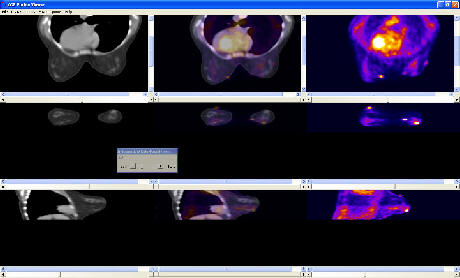
\includegraphics[width=10cm]{images/multimodalbreastimage}~\\
\caption{\label{fig:screenshot}A screenshot of a fused data set.
}
\end{figure}

The growing interest in multimodal interface development is inspired in large part by goals of supporting more flexible, transparent, efficient and powerfully expressive means of human-computer interaction than in the past. Multimodal interfaces are expected to support a wider range of diverse applications, be usable by a broader spectrum of the average population, and function more reliably under realistic and challenging usage conditions.

Computer-aided  diagnosis  often  implies  processing large and high dimensional datasets, for instance, high-resolution volumes containing millions of voxels.

Visualisation and analysis of such data can be very time demanding for physicians but also very computationally expensive for machines assisting diagnosis tasks. Fortunately, in many cases the relevant information for an application can be represented in lower dimensional spaces. If appropriately  chosen and designed, dimensionality reduction methods will not only decrease the processing time but also facilitate any posterior analysis. Therefore, they can be of great use to a variety of CAD (Computer Aided Diagnosis)  applications, ranging  from  general problems such as classification and visualisation, to more specific ones like multi-modal registration or motion compensation.

Dimensionality reduction in CAD has relied mainly on linear methods and linear  methods  are  however not suitable for handling non-linear complex relationships among the data samples. Non-linear approaches based on manifold learning are a good alternative for dimensionality reduction in such cases.

Medical Imaging Multimodality Breast Cancer Diagnosis User Interface (MIMBCD-UI)  registration  consists  in  finding  a map between images of the same scene acquired with different imaging modalities. The standard approach to multi-modal registration is to use sophisticated similarity metrics such as mutual information to compare the images.

%TEX root = ../dissertation.tex

\chapter{Overview}
\label{chapter:overview}

CAD Based-Systems are typically single-user oriented that is, designed to support individual tasks such as notations and information visualisation. This personal and task-oriented approach for clinical software provides little support for the aggregation of resources and tools required in carrying out higher level activities for multimodality of medical imaging. It is left to the user to aggregate such resources and tools in meaningful bundles according to the activity at hand, and users often have to reconfigure this aggregation manually when shifting between a set of parallel activities and machines.

A  suited  number  of  studies  have  shown  that  clinical  professionals, upon the act of organising and thinking in their work routines, which often carried out search of general objectives, often in collaboration with others \cite{Bardram04realtimecollaboration, citeulike:1090639, Mark05notask}, are significant mental and manual overhead associated with handling of  parallel  work  and  interruptions \cite{Czerwinski04adiary, Smith03groupbar:the}. The rest of the user  interfaces  in  the  current operating systems, fail to provide adequate support in the resumption of the previous  activities  and  for an  easy  switching  between  parallel  activities \cite{Robertson04scalablefabric:, Robertson00thetask}.

Clinical user interfaces have been extensively discussed in the literature on information visualisation. MIMBCD-UI shows the details of an user interface for diagnosing breast cancer using multimodality medical imaging.

MIMBCD-UI have several benefits. In fact, the diagnosis it self is more efficient since the clinical users may navigate using the overview of multimodality of imaging rather than the others techniques. The overview of multimodality of imaging window aids users in keeping track of their current position in the information space \cite{plaisant1994image}. Moreover the overview window itself give users task-relevant information and a feeling of control \cite{shneiderman1987designing}.

A multimodality of views permits to acquire better, more efficient and flexible information and to easily diagnose in it; however, it is more difficult to users to manage information in a more complex user interface.

Specifically, this project deals with the use of a recently proposed technique in literature: Deep Convolutional Neural Networks (CNNs).

These deep networks will incorporate information from several different modes: \gls{MRI}, \gls{US} images, \gls{MG} images (both views CC and MLO) and text.

The proposed algorithm, called for multimodality CNNs (MMCNNs) will have the ability to process multimodal information at an unified and sustained manner.

This methodology needs to "learn" what are the masses and calcifications.

So that is necessary to collect the ground truth, or notes of the masses and calcifications provided by medical experts.

\break

For the collection of these notes, the design and development of an interface is necessary allows the user (in this case, the medical specialist) to display various types of image (i.e., \gls{US}, \gls{MRI} and \gls{MG}), and that also allows for user interaction, particularly in providing the notes of the masses and calcifications.

For these reasons, it is crucial for the development of this project, cooperation with experts providing the above notes.
%!TEX root = ../dissertation.tex

\chapter{Conclusion}
\label{chapter:conclusion}

There is a lot of information concerning work in development for clinical user interfaces on images tools views, but, in fact, there is little in multimodality image and its display in breast cancer diagnosis fields.

This master project report is a first essay, to what will be the master thesis related work dissertation and state of the art \cite{borchers2012persuasion}. It describe related systems that have been designed to provide more direct support and fundament to our research. We follow at most clinical imaging tools and personal computer-based interfaces as well as a hypothetical solution of implementation with mobile interfaces where it can help us understand the right user interface solution.

In short, we analyse and rehearsed what was the first approach to the subject-matter literature on a state of the art milestone of the project to understand and to investigate the various innovations and topics made in this field of research.

So far, there have been hardly any specific studies wherein the medical interfaces are tested and evaluated for their comprehensibility and usability to users. Pretty interfaces that hide the ugly reality of underlying data do not engender clinician trust and respect. New visual cues that provide immediate user insight into assumptions and deficiencies regarding the displayed information are required. Clinicians expect and interface to keep clear and direct with easy and intuitive usability.

Some requirements for advancing innovative imaging multimodality are not just intellectual ones, but rather social, political, and educational in nature. The development of state-of-the-art of multimodal images user interface of this kind also requires multidisciplinary expertise in a variety of areas, such as human factors and ergonomics \cite{wikipedia2016humanfactors}, perception and graphics, linguistics, psychology, pattern recognition, statistics, engineering and computer science. The multidisciplinary nature of this research across the entire spectrum.

A review of the state of the art in the field is provided showing the increasing interest of researchers in the domain and a wide range applications where these methods can be applied.

Cancer is projected to become the world's leading cause of death by 2016, with the burden of disease shifting further towards medically underserved populations in industrialised countries and the developing world.

New approaches are required across the spectrum of cancer management, in prevention, diagnosis, treatment, education and care. If developed and tested appropriately, optical imaging technologies can play an important role in several aspects, from providing objective diagnostic screening at the community healthcare level, to enabling pathology guidance in the clinical setting.

Importantly, by delivering these technical capabilities within cost-effective platforms, the impact on public health can be magnified through expanding patient access to previously unreachable healthcare systems.


\bibliographystyle{ieeetr}
\addcontentsline{toc}{chapter}{Bibliography}
\bibliography{bibliography/dissertation}

% Appendix
\appendix
%!TEX root = ../dissertation.tex

% Entry point for chapters
% In this file you define the order
% in which the chapters are included

% Chapters
%!TEX root = ../dissertation.tex

\chapter{Introduction}
\label{chapter:introduction}

The Medical Imaging Multimodality Breast Cancer Diagnosis is a topic of great interest, it has been the subject of intensive research in the world of medicine. However the developments in terms of innovation in the computational world are still scarce. The Interface herein proposer deals with the processing and analysis of images. Indeed, this topic has a wide spectrum of applications raging from video surveillance based systems to medical applications.

In the proposed work, i.e., the analysis mammography using multi-modality images, several issues must be considered. First each image modality has its own image features. Which must be included in the interface. Second, for each image modality several and distinct image feature must be considered.

Masses and calcifications can be accurately diagnosed from cytological features [1] of the cells that constitute them. However, the diagnostic accuracy depends on the training, experience, and many indefinite factors of interpretation of the medical expert in cytological evaluation.

There were, in fact, some developments in the past facing the Computer-Based classification system [2, 3] that assists in the diagnosis of breast cells based on visual assessment of characteristics of the cells. [4] A set of cytologic features, previously evaluated visually, are now replaced by digital ones, evaluated by image analysis. In this project, the interface will be used by several experts in the field, to collect the ground truth, for Mammograms, MRI and Ultrasounds images. Those mammography experts annotations will be a crucial step towards the performance evaluation of Machine Learning (ML) Based-Algorithms.

Doctors are accountable for decisions they make on behalf of their patients. Likewise, computer interface developers and engineers must assume accountability for limitations, assumptions and other unplanned deficiencies that impact on the integrity, validity, quantity and timeliness of data made accessible through their interfaces.

Art and science [5] applied to the user interface filed of clinical care are based on an unusual combination of non-judgement trust and exasperating mistrust [6]. Two major obstacles to good clinicians-patient communication are differences of language and culture [7]. Doctors and clinicians require that theirs patients keep no secrets or else an opportunity to reach the right diagnosis or select the proper therapy may be lost. At the same time, doctors and clinicians are taught to question everything they hear from both colleagues and patients. It is deeply ingrained in medical training to make no important decisions based on information supplied solely by others. The highly trained mistrust explains why many times patients complained that a dozen different people asked the same question. A deeply ingrained aversion to secrets and lies greatly characterise a clinician’s attitude toward a computer interface where the responsibility of interface developers address and incorporate the concept of visual accountability extending well beyond medical user interfaces.

\clearpage

% Commands to include a figure:
\begin{figure}[!hbt]
\centering
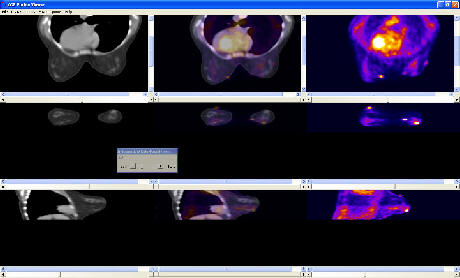
\includegraphics[width=10cm]{images/multimodalbreastimage}~\\
\caption{\label{fig:screenshot}A screenshot of a fused data set.
}
\end{figure}

The growing interest in multimodal interface development is inspired in large part by goals of supporting more flexible, transparent, efficient and powerfully expressive means of human-computer interaction than in the past. Multimodal interfaces are expected to support a wider range of diverse applications, be usable by a broader spectrum of the average population, and function more reliably under realistic and challenging usage conditions.

Computer-aided  diagnosis  often  implies  processing large and high dimensional datasets, for instance, high-resolution volumes containing millions of voxels.

Visualisation and analysis of such data can be very time demanding for physicians but also very computationally expensive for machines assisting diagnosis tasks. Fortunately, in many cases the relevant information for an application can be represented in lower dimensional spaces. If appropriately  chosen and designed, dimensionality reduction methods will not only decrease the processing time but also facilitate any posterior analysis. Therefore, they can be of great use to a variety of CAD (Computer Aided Diagnosis)  applications, ranging  from  general problems such as classification and visualisation, to more specific ones like multi-modal registration or motion compensation.

Dimensionality reduction in CAD has relied mainly on linear methods and linear  methods  are  however not suitable for handling non-linear complex relationships among the data samples. Non-linear approaches based on manifold learning are a good alternative for dimensionality reduction in such cases.

Medical Imaging Multimodality Breast Cancer Diagnosis User Interface (MIMBCD-UI)  registration  consists  in  finding  a map between images of the same scene acquired with different imaging modalities. The standard approach to multi-modal registration is to use sophisticated similarity metrics such as mutual information to compare the images.

%TEX root = ../dissertation.tex

\chapter{Overview}
\label{chapter:overview}

CAD Based-Systems are typically single-user oriented that is, designed to support individual tasks such as notations and information visualisation. This personal and task-oriented approach for clinical software provides little support for the aggregation of resources and tools required in carrying out higher level activities for multimodality of medical imaging. It is left to the user to aggregate such resources and tools in meaningful bundles according to the activity at hand, and users often have to reconfigure this aggregation manually when shifting between a set of parallel activities and machines.

A  suited  number  of  studies  have  shown  that  clinical  professionals, upon the act of organising and thinking in their work routines, which often carried out search of general objectives, often in collaboration with others \cite{Bardram04realtimecollaboration, citeulike:1090639, Mark05notask}, are significant mental and manual overhead associated with handling of  parallel  work  and  interruptions \cite{Czerwinski04adiary, Smith03groupbar:the}. The rest of the user  interfaces  in  the  current operating systems, fail to provide adequate support in the resumption of the previous  activities  and  for an  easy  switching  between  parallel  activities \cite{Robertson04scalablefabric:, Robertson00thetask}.

Clinical user interfaces have been extensively discussed in the literature on information visualisation. MIMBCD-UI shows the details of an user interface for diagnosing breast cancer using multimodality medical imaging.

MIMBCD-UI have several benefits. In fact, the diagnosis it self is more efficient since the clinical users may navigate using the overview of multimodality of imaging rather than the others techniques. The overview of multimodality of imaging window aids users in keeping track of their current position in the information space \cite{plaisant1994image}. Moreover the overview window itself give users task-relevant information and a feeling of control \cite{shneiderman1987designing}.

A multimodality of views permits to acquire better, more efficient and flexible information and to easily diagnose in it; however, it is more difficult to users to manage information in a more complex user interface.

Specifically, this project deals with the use of a recently proposed technique in literature: Deep Convolutional Neural Networks (CNNs).

These deep networks will incorporate information from several different modes: \gls{MRI}, \gls{US} images, \gls{MG} images (both views CC and MLO) and text.

The proposed algorithm, called for multimodality CNNs (MMCNNs) will have the ability to process multimodal information at an unified and sustained manner.

This methodology needs to "learn" what are the masses and calcifications.

So that is necessary to collect the ground truth, or notes of the masses and calcifications provided by medical experts.

\break

For the collection of these notes, the design and development of an interface is necessary allows the user (in this case, the medical specialist) to display various types of image (i.e., \gls{US}, \gls{MRI} and \gls{MG}), and that also allows for user interaction, particularly in providing the notes of the masses and calcifications.

For these reasons, it is crucial for the development of this project, cooperation with experts providing the above notes.
%!TEX root = ../dissertation.tex

\chapter{Conclusion}
\label{chapter:conclusion}

There is a lot of information concerning work in development for clinical user interfaces on images tools views, but, in fact, there is little in multimodality image and its display in breast cancer diagnosis fields.

This master project report is a first essay, to what will be the master thesis related work dissertation and state of the art \cite{borchers2012persuasion}. It describe related systems that have been designed to provide more direct support and fundament to our research. We follow at most clinical imaging tools and personal computer-based interfaces as well as a hypothetical solution of implementation with mobile interfaces where it can help us understand the right user interface solution.

In short, we analyse and rehearsed what was the first approach to the subject-matter literature on a state of the art milestone of the project to understand and to investigate the various innovations and topics made in this field of research.

So far, there have been hardly any specific studies wherein the medical interfaces are tested and evaluated for their comprehensibility and usability to users. Pretty interfaces that hide the ugly reality of underlying data do not engender clinician trust and respect. New visual cues that provide immediate user insight into assumptions and deficiencies regarding the displayed information are required. Clinicians expect and interface to keep clear and direct with easy and intuitive usability.

Some requirements for advancing innovative imaging multimodality are not just intellectual ones, but rather social, political, and educational in nature. The development of state-of-the-art of multimodal images user interface of this kind also requires multidisciplinary expertise in a variety of areas, such as human factors and ergonomics \cite{wikipedia2016humanfactors}, perception and graphics, linguistics, psychology, pattern recognition, statistics, engineering and computer science. The multidisciplinary nature of this research across the entire spectrum.

A review of the state of the art in the field is provided showing the increasing interest of researchers in the domain and a wide range applications where these methods can be applied.

Cancer is projected to become the world's leading cause of death by 2016, with the burden of disease shifting further towards medically underserved populations in industrialised countries and the developing world.

New approaches are required across the spectrum of cancer management, in prevention, diagnosis, treatment, education and care. If developed and tested appropriately, optical imaging technologies can play an important role in several aspects, from providing objective diagnostic screening at the community healthcare level, to enabling pathology guidance in the clinical setting.

Importantly, by delivering these technical capabilities within cost-effective platforms, the impact on public health can be magnified through expanding patient access to previously unreachable healthcare systems.


% Glossary and Acronym List
\if\includeGlossary 1
\printglossary
\fi

% Back Cover
\pagenumbering{gobble}
\NewPage

\end{document}
